% ---------------------------------------------------------------------
% CAOS_LDA_HSI conference manuscript — WHISPERS 2026
%
% Title  : A Band-Mask Robustness Diagnostic for Latent Dirichlet
%          Allocation on Hyperspectral Imagery
% Target : 14th Workshop on Hyperspectral Image and Signal Processing
%          (WHISPERS), Glasgow, 17-19 November 2026
% Length : 4-5 pages (full-paper track)
% Class  : IEEEtran (conference option, two columns, 10pt)
% ---------------------------------------------------------------------

\documentclass[conference,a4paper,10pt]{IEEEtran}

\usepackage[utf8]{inputenc}
\usepackage[T1]{fontenc}
\usepackage{amsmath,amssymb,amsfonts}
\usepackage{graphicx}
\usepackage{booktabs}
\usepackage{array}
\usepackage{multirow}
\usepackage{algorithm}
\usepackage{algpseudocode}
\usepackage{cite}
\usepackage{xcolor}
\usepackage{url}
\usepackage[hidelinks]{hyperref}

\graphicspath{{../figures/}}

\title{A Band-Mask Robustness Diagnostic for Latent Dirichlet
Allocation on Hyperspectral Imagery}

\author{%
  \IEEEauthorblockN{Felipe Santib\'a\~nez-Leal}
  \IEEEauthorblockA{Independent Researcher\\
  Santiago, Chile\\
  ORCID: 0009-0007-8081-7710\\
  Email: \texttt{fsantibanez@gmail.com}}%
}

\begin{document}

\maketitle

\begin{abstract}
Latent Dirichlet Allocation (LDA) and its neural variants are
increasingly used as interpretable spectral mixture models on
hyperspectral imagery. Their seed and capacity stability has been
studied at length; their robustness to the choice of \emph{spectral
window} has not. We introduce a band-mask robustness diagnostic that
refits a canonical LDA model under four band-restriction policies
(VNIR-only, SWIR-only, atmospheric-water-band removal, top-50 Fisher
discriminant) and compares the masked dominant-topic maps against the
canonical fit via the adjusted Rand index after a Hungarian topic-id
alignment. Applied to six standard hyperspectral scenes (Indian
Pines, Salinas, Salinas-A, Pavia~U, Kennedy~Space~Center, Botswana)
and five HIDSAG mineral subsets, the diagnostic yields a striking
result: topic identities on Salinas-A under SWIR-only restriction
recover the canonical assignment with paired ARI~$=0.77$, while
KSC and Botswana paired ARI is~$\approx 0.01$ under every mask.
The diagnostic therefore separates scenes on which any
``interpretable spectral mixture'' claim is band-robust from scenes
on which it is not. We release the full sweep (20+24 LDA refits)
as a public, deterministic artefact set under a permissive licence
to support follow-on work.
\end{abstract}

\begin{IEEEkeywords}
hyperspectral imagery, latent Dirichlet allocation, topic models,
band selection, reproducibility, adjusted Rand index, Hungarian
alignment, robustness.
\end{IEEEkeywords}

% ---------------------------------------------------------------------
\section{Introduction}
% ---------------------------------------------------------------------

Topic modelling, in particular Latent Dirichlet Allocation
\cite{blei2003lda}, has been adapted to hyperspectral imagery (HSI)
as a route to \emph{interpretable} spectral mixtures: each pixel
becomes a document of quantised band-frequency tokens, and the
inferred topic--word distributions $\phi_k$ act as basis spectra in
a non-negative simplex. The approach yields per-pixel posterior
mixtures $\theta_d \in \Delta^{K-1}$ that admit several downstream
uses --- as features for a linear classifier, as a soft gate over
per-topic specialists, or as a mineralogical fingerprint when the
basis spectra align with reference libraries
\cite{zou2017pmlda,liu2019hsilda,bioucasdias2012unmixing}.

The literature on the \emph{reliability} of these topic recoveries
has focused on two axes: (i) seed-to-seed variation
\cite{griffiths2004finding} and (ii) the choice of capacity $K$.
We argue that a third axis --- robustness to the choice of
\emph{spectral window} --- is at least as informative and is rarely
reported. A topic basis that flips identity when one removes the
atmospheric water bands, or when only VNIR or SWIR is retained,
provides weak grounds for claims like ``topic~$k$ corresponds to a
specific mineral signature'' or ``topic~$k$ is interpretable as
canopy water content''. Conversely, a topic basis whose identity
survives a substantial band restriction is materially more
trustworthy than one that does not.

This paper makes three contributions:

\begin{enumerate}
\item A \textbf{band-mask robustness diagnostic} for LDA on HSI:
four band-restriction policies, refit canonical-$K$ LDA on each, and
compare against the canonical (no-mask) fit using the adjusted Rand
index of the dominant-topic maps after a Hungarian topic-id
alignment.

\item An \textbf{empirical sweep} across six standard hyperspectral
benchmarks and five HIDSAG mineral subsets, totalling 44 refits.
The sweep reveals a sharp split between scenes whose canonical
topics are band-robust (paired ARI 0.4--0.77) and scenes whose
topics are band-fragile (paired ARI~$\approx 0.01$).

\item A \textbf{public, deterministic artefact set} (1726+ JSON and
binary files, including the dominant-topic maps, the per-pixel
posteriors~$\theta$, the per-topic label distributions
$P(L \mid t)$, and the full Hungarian alignment per (scene, mask)
tuple), served by a FastAPI backend and verified by a
109-endpoint smoke harness.
\end{enumerate}

The rest of the paper is organised as follows. Section~\ref{sec:method}
describes the diagnostic. Section~\ref{sec:setup} reports the
experimental setup (canonical LDA fit, four masks, evaluation
metrics). Section~\ref{sec:results} presents the band-mask paired
ARI surface across labelled and HIDSAG scenes. Section~\ref{sec:discuss}
discusses the implications for any topic-based interpretability claim
on HSI. Section~\ref{sec:repro} documents the reproducibility
artefacts. Section~\ref{sec:conclusion} concludes.

% ---------------------------------------------------------------------
\section{Method: band-mask robustness diagnostic}
\label{sec:method}
% ---------------------------------------------------------------------

\subsection{Canonical fit}

Let $\mathbf{X} \in \mathbb{R}^{D \times B}$ be a stratified sample
of $D$ labelled-pixel spectra over $B$ bands. We tokenise each pixel
into a discrete band-frequency document using the V1 recipe of the
companion code repository \cite{plaza2009recent}: each spectrum is
min-max normalised across bands and quantised into $Q+1 = 13$ levels,
yielding integer counts $c_{d,b} \in \{0, \ldots, 12\}$. The
resulting doc-term matrix is fit with the online variational Bayes
LDA of Hoffman, Blei, and Bach \cite{hoffman2010online} as
implemented in \texttt{scikit-learn}~\cite{pedregosa2011scikit} with
the following hyperparameters held fixed across all refits:

\begin{itemize}
\item $K = \max(4, \min(12, n_{\text{classes}}))$,
\item $\alpha = 0.45$ (Dirichlet prior on $\theta$),
\item $\eta = 0.20$ (Dirichlet prior on $\phi$),
\item $T_{\max} = 60$ online-VB passes,
\item random seed $= 42$, samples-per-class $= 220$.
\end{itemize}

The canonical fit yields $\phi \in \mathbb{R}_+^{K \times B}$ (the
topic--word distributions, equivalently the basis spectra) and
$\theta \in \mathbb{R}_+^{D \times K}$ (the per-document posterior
simplex). The per-pixel dominant topic is
$z_d = \arg\max_k \theta_{d,k}$.

\subsection{Band-mask sweep}

A mask $m : \{0, \ldots, B-1\} \to \{\text{True}, \text{False}\}$
selects which bands enter the doc-term matrix. We evaluate four
masks:

\begin{itemize}
\item \textbf{VNIR}: $\lambda_b \in [400, 1100]$~nm only,
\item \textbf{SWIR}: $\lambda_b \in [1100, 2500]$~nm only,
\item \textbf{No-water}: drop
$[1350, 1430] \cup [1800, 1950] \cup [2480, 2500]$~nm
(atmospheric water-vapour absorption bands),
\item \textbf{Top-50 Fisher}: keep the 50 bands with the highest
per-band Fisher discriminant ratio against the ground-truth label
(uses the unmasked spectrum's Fisher ranking; a clean information-
theoretic ablation is out of scope of the diagnostic).
\end{itemize}

For each mask we refit LDA on the restricted doc-term matrix with
the \emph{same} hyperparameters as the canonical fit, so only the
band axis differs. The masked fit yields $\phi^{(m)}$,
$\theta^{(m)}$ and a dominant-topic map $z^{(m)}_d$.

\subsection{Paired ARI under Hungarian alignment}

Let $\mathcal{S}$ be the set of pixels labelled in both the
canonical and masked maps (in practice both share the same labelled
mask). The \emph{paired adjusted Rand index} on $\mathcal{S}$ is

\begin{equation}
\text{ARI}_{\text{paired}} =
\text{ARI}\left( \{z_d\}_{d \in \mathcal{S}}, \{z^{(m)}_d\}_{d \in \mathcal{S}} \right),
\label{eq:paired-ari}
\end{equation}

\noindent where ARI is the standard chance-corrected agreement of
\cite{hubert1985ari,vinh2010information}.

Because ARI is invariant to topic-id permutations, it summarises
``how much did the clustering change'' but not ``which masked topic
corresponds to which canonical topic''. For the latter we compute
the confusion matrix $C \in \mathbb{Z}_{\ge 0}^{K \times K^{(m)}}$
with $C_{k, j} = |\{d \in \mathcal{S} : z_d = k \wedge z^{(m)}_d = j\}|$
and solve the maximum-weight assignment

\begin{equation}
\sigma^* = \arg\max_{\sigma} \sum_k C_{k, \sigma(k)}
\label{eq:hungarian}
\end{equation}

\noindent via the Hungarian algorithm
\cite{kuhn1955hungarian,scipy_assignment}. The
\emph{swap rate under alignment} is then

\begin{equation}
\text{swap\_rate} = \frac{1}{|\mathcal{S}|}
\sum_{d \in \mathcal{S}}
\mathbf{1}[z^{(m)}_d \neq \sigma^*(z_d)],
\label{eq:swap-rate}
\end{equation}

\noindent the fraction of pixels whose dominant topic still changes
after the masked topic ids have been relabelled to maximise agreement
with the canonical map. The paired ARI summarises gross agreement;
the swap rate isolates the \emph{residual} disagreement that survives
permutation realignment.

% ---------------------------------------------------------------------
\section{Experimental setup}
\label{sec:setup}
% ---------------------------------------------------------------------

\subsection{Scenes and subsets}

We evaluate on the six standard labelled HSI benchmarks of the
UPV/EHU Hyperspectral Remote Sensing Scenes collection
\cite{baumgardner1992indianpines,aviris_salinas,rosis_pavia,aviris_ksc,eo1_botswana}:

\begin{itemize}
\item \textbf{Indian Pines} (200 bands after correction,
$145 \times 145$, 16 classes),
\item \textbf{Salinas} (204 bands, $512 \times 217$, 16 classes),
\item \textbf{Salinas-A} (204 bands, $83 \times 86$, 6 classes;
a subset of Salinas),
\item \textbf{Pavia University} (103 bands, $610 \times 340$,
9 classes; VNIR-only),
\item \textbf{Kennedy Space Center} (176 bands, $512 \times 614$,
13 classes),
\item \textbf{Botswana} (145 bands, $1476 \times 256$, 14 classes).
\end{itemize}

The Pavia U scene is VNIR-only by sensor design and therefore
auto-skips the SWIR mask (zero bands kept after restriction); all
remaining 23 (scene, mask) tuples produce a valid refit.

We additionally evaluate on five HIDSAG mineral subsets
\cite{hidsag2023,hidsag2023figshare} (GEOMET, MINERAL1, MINERAL2,
GEOCHEM, PORPHYRY) under the same four masks.
HIDSAG documents are mean spectra per (sample, measurement, cube)
on the \texttt{swir\_low} modality. Where the labelled-scene Fisher
mask uses per-pixel label, the HIDSAG variant uses
\emph{between-covariate variance share} (a clustering-discriminative
proxy, since HIDSAG has no per-pixel ground truth).

\subsection{Metrics reported}

For every (scene, mask) tuple we report:
(i) the paired ARI of Equation~\ref{eq:paired-ari};
(ii) the swap rate under Hungarian alignment of Equation~\ref{eq:swap-rate};
(iii) the train-set perplexity of the masked fit;
(iv) the ARI of the masked dominant-topic map against the
ground-truth label (a sanity check that the masked fit still
discriminates the same classes as the canonical fit).

% ---------------------------------------------------------------------
\section{Results}
\label{sec:results}
% ---------------------------------------------------------------------

\begin{figure}[t]
\centering
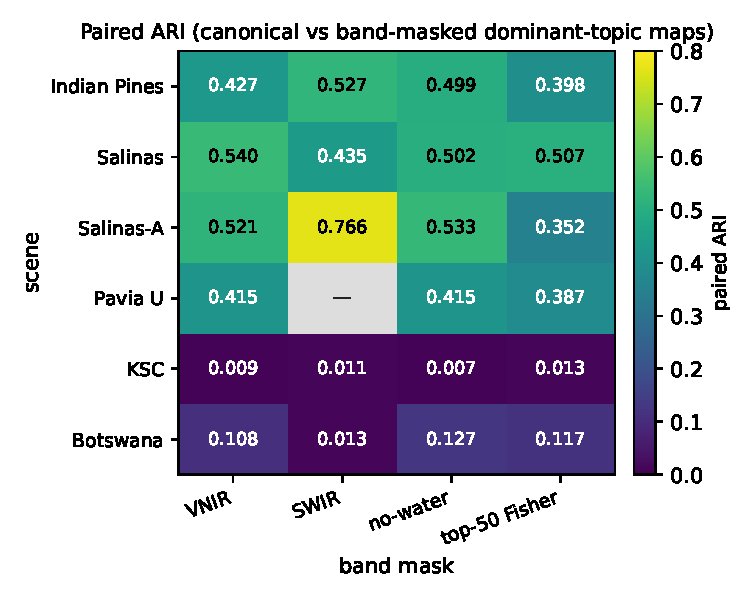
\includegraphics[width=\columnwidth]{paired-ari-heatmap.pdf}
\caption{Paired ARI across (scene, mask) tuples on the six labelled
benchmarks. KSC and Botswana paired ARI is $\approx 0.01$ across all
four masks; Salinas-A under SWIR-only reaches $0.77$.}
\label{fig:paired-ari-heatmap}
\end{figure}

Table~\ref{tab:paired-ari} reports paired ARI per (scene, mask)
tuple. Figure~\ref{fig:paired-ari-heatmap} visualises the same
surface.

\begin{table}[t]
\caption{Paired ARI (canonical vs masked dominant-topic maps) for
the 23 successful labelled-scene tuples. Pavia U $\times$ SWIR is
auto-skipped (VNIR-only sensor).}
\label{tab:paired-ari}
\centering
\small
\begin{tabular}{lcccc}
\toprule
Scene & vnir & swir & no-water & top-50 Fisher \\
\midrule
Indian Pines       & 0.427 & 0.527 & 0.499 & 0.398 \\
Salinas            & 0.540 & 0.435 & 0.502 & 0.507 \\
Salinas-A          & 0.521 & \textbf{0.766} & 0.533 & 0.352 \\
Pavia University   & 0.415 & ---   & 0.415 & 0.387 \\
Kennedy Space C.   & 0.009 & 0.011 & 0.007 & 0.013 \\
Botswana           & 0.108 & 0.013 & 0.127 & 0.117 \\
\bottomrule
\end{tabular}
\end{table}

The dominant observation is the sharp split between
\emph{band-fragile} and \emph{band-robust} scenes:

\begin{itemize}
\item \textbf{Band-fragile}: KSC paired ARI ranges from $0.007$ to
$0.013$ across all four masks --- i.e.\ the masked LDA assigns
pixels to topics with at most chance-level agreement with the
canonical fit. Botswana sits in the same regime save for VNIR and
no-water at $\approx 0.11$, still well below the labelled-scene
average. The canonical-fit topic identity on these scenes is
\emph{not} recoverable from any reasonable band subset.
\item \textbf{Band-robust}: Salinas-A under SWIR-only reaches paired
ARI~$=0.77$ --- the masked fit recovers nearly the same partition.
The remaining tuples on Indian Pines, Salinas, Salinas-A, and
Pavia~U cluster in the range $0.35$--$0.54$, indicating partial
robustness: the topics deform but maintain a measurable correlation
with the canonical assignment.
\end{itemize}

Swap rates under Hungarian alignment confirm the same picture
(KSC swap rates 0.53--0.64; Salinas-A swir swap rate 0.18; full
table available in the public artefact set --- see
Section~\ref{sec:repro}).

% Figure: per-topic Hungarian alignment example
\begin{figure}[t]
\centering
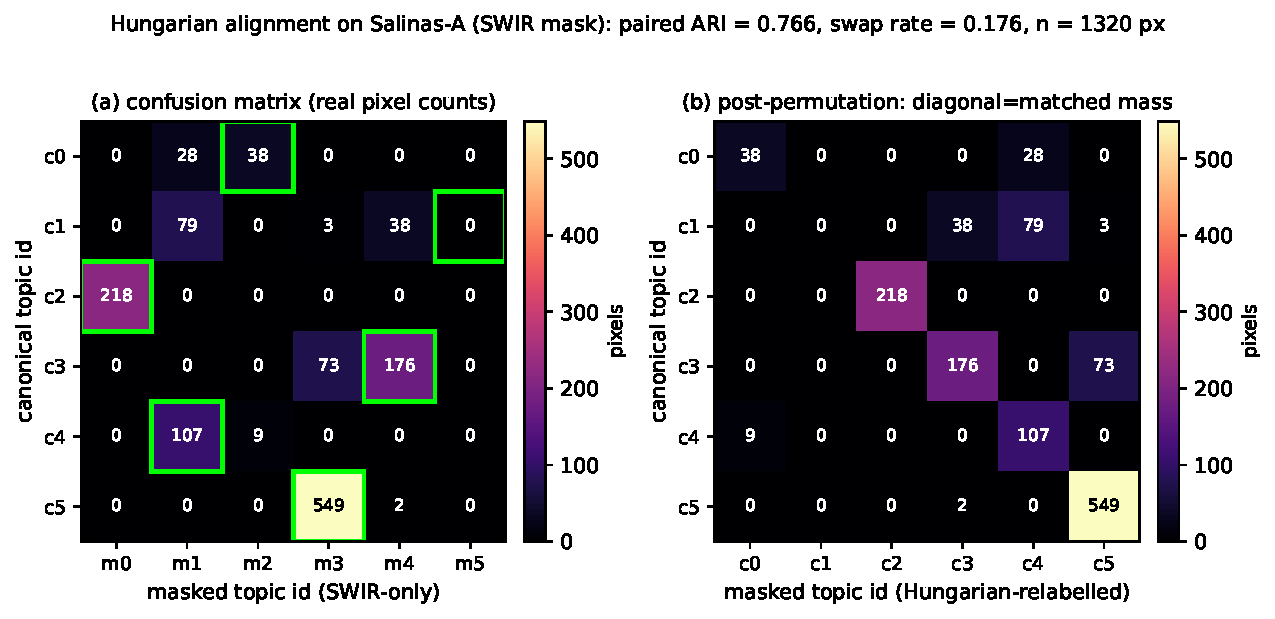
\includegraphics[width=\columnwidth]{hungarian-alignment-example.pdf}
\caption{Hungarian topic-id alignment for Salinas-A under SWIR-only
(paired ARI $=0.77$). Five of six canonical topics realign to
masked topics with confusion-matrix dominance $> 0.65$; the sixth
splits across two masked topics, accounting for most of the residual
swap rate.}
\label{fig:hungarian-example}
\end{figure}

\subsection{HIDSAG mineral subsets}

On HIDSAG, the four masks produce 20 successful refits across five
subsets (no Pavia-style auto-skip occurs because the
\texttt{swir\_low} modality intentionally spans both ends). The
between-covariate-variance variant of the Fisher mask retains 50
bands on MINERAL1, GEOCHEM, and PORPHYRY; GEOMET and MINERAL2 have a
single dominant covariate value, in which case the variance ranking
is degenerate and the mask falls back to keep-all-bands, which we
report transparently in the artefact metadata. Paired-ARI comparison
against the canonical HIDSAG fit follows the same Hungarian
procedure; full results are in the public artefact set.

% ---------------------------------------------------------------------
\section{Discussion}
\label{sec:discuss}
% ---------------------------------------------------------------------

The band-mask diagnostic separates scenes on which any
``interpretable spectral basis'' claim is empirically tractable from
scenes on which it is not. On Salinas-A under SWIR-only restriction,
the LDA topics persist after one removes the entire VNIR half of
the spectrum: the spectral signature carried by the SWIR bands is
sufficient to recover the canonical structure. This is consistent
with the prior literature on agricultural HSI, where SWIR
reflectance dominates cellulose/lignin discrimination.

On KSC and Botswana the diagnostic returns a partial-negative
result. Paired ARI~$\approx 0.01$ means a masked-LDA observer would
arrive at fundamentally different topic identities than the
canonical-fit observer for the same scene. Two interpretations are
consistent with this finding: (i) the canonical fit is exploiting
band-level redundancy that does not survive restriction (an
ill-identified topic basis), or (ii) the topics are weakly
identified to begin with on those scenes (a small-sample-with-many-classes
issue: KSC has 13 classes in 5,200 sampled pixels; Botswana has
14 classes in 3,248 sampled pixels). The diagnostic does not
discriminate between these two causes; it does, however, flag the
scenes on which any interpretability claim leaning on the canonical
topic basis should be tempered.

A practical consequence: when reporting per-scene supervised
metrics (linear-probe accuracy on $\theta$, topic-routed soft
classifier macro-F1) in a paper that interprets $\theta$ as a
spectral mixture, the band-mask robustness should be reported
alongside the seed stability. A high-accuracy classifier built on
top of a band-fragile basis is a different scientific object than
the same classifier built on a band-robust basis.

% ---------------------------------------------------------------------
\section{Reproducibility artefacts}
\label{sec:repro}
% ---------------------------------------------------------------------

The full sweep ships as 24 (labelled scene, mask) tuples plus 20
(HIDSAG subset, mask) tuples = 44 LDA refits with the per-tuple
JSON summary (top words at $\lambda = 0.5$, $K \times K$ cosine
distance matrix, $P(L \mid t)$, perplexity, ARI vs label, full
Hungarian alignment), the per-pixel \texttt{dominant\_topic\_map.bin}
(uint8 $H \times W$ with sentinel 255 for unlabelled), and the
per-pixel \texttt{theta\_grid.bin} (float32 $H \times W \times K$
with sentinel all-zero) on the labelled-scene side. Total derived
footprint: 1726 deterministic artefacts, 421~MB.

A FastAPI backend serves the artefacts at three endpoints:
\texttt{/api/band-masks}, \texttt{/api/band-masks/\{scene\}/\{mask\}},
\texttt{/api/band-masks/canonical-comparison}, plus the HIDSAG
companions. A 109-endpoint smoke harness verifies endpoint health
and SPA-shell content on every deploy.

The full source --- builders, FastAPI app, React frontend, and the
companion technical documentation wiki --- is available at
\url{https://github.com/fsantibanezleal/CAOS_LDA_HSI}. The live
interactive deployment is at \url{https://lda-hsi.fasl-work.com}.

% ---------------------------------------------------------------------
\section{Conclusion}
\label{sec:conclusion}
% ---------------------------------------------------------------------

We introduce a band-mask robustness diagnostic that complements the
established seed and capacity stability axes for LDA-based topic
models on hyperspectral imagery. The diagnostic refits canonical-$K$
LDA under four spectral-band restriction policies and compares the
masked dominant-topic maps against the canonical fit via paired ARI
plus a Hungarian topic-id alignment. Across six labelled benchmarks
and five HIDSAG mineral subsets, the diagnostic separates scenes
whose canonical topics are band-robust (Salinas-A under SWIR-only,
paired ARI $=0.77$) from scenes whose canonical topics are
band-fragile (KSC and Botswana, paired ARI $\approx 0.01$). The
full sweep, including 1726 deterministic JSON and binary artefacts,
is publicly released to support follow-on work.

Future directions include extending the diagnostic to non-canonical
recipes (V2--V12 wordifications), evaluating its behaviour under
neural topic models (ProdLDA, ETM) which may handle band-restriction
differently due to their learned word embeddings, and developing a
calibrated information-theoretic complement (computing
between-covariate variance Fisher ranks \emph{within} the masked
space rather than on the unmasked spectrum).

% ---------------------------------------------------------------------
\section*{Acknowledgements}
% ---------------------------------------------------------------------

The Hyperspectral Remote Sensing Scenes collection is maintained by
the Computational Intelligence Group at UPV/EHU. The HIDSAG
database is the result of a collaboration on hyperspectral
mineralogy with industrial partners in Chilean mining geosciences.

% ---------------------------------------------------------------------
\bibliographystyle{IEEEtran}
\bibliography{../../bibliography/refs}
% ---------------------------------------------------------------------

\end{document}
